\documentclass[12pt, a4paper, twoside]{report}

% --- PAKIETY ---
\usepackage[utf8]{inputenc}
\usepackage[T1]{fontenc}
\usepackage[polish]{babel}
\usepackage{amsmath, amsfonts, amssymb} % Matematyka
\usepackage{graphicx} % Obrazki
\usepackage{hyperref} % Aktywne linki
\usepackage{geometry} % Marginesy
\usepackage{epigraph}
\setlength{\epigraphwidth}{0.7\textwidth}
\geometry{margin=2.5cm}

% --- USTAWIENIA DLA KODU ŹRÓDŁOWEGO (Python/Bash) ---
\usepackage{listings}
\usepackage{xcolor}

\definecolor{codegreen}{rgb}{0,0.6,0}
\definecolor{codegray}{rgb}{0.5,0.5,0.5}
\definecolor{codepurple}{rgb}{0.58,0,0.82}
\definecolor{backcolour}{rgb}{0.95,0.95,0.92}

\lstdefinestyle{mystyle}{
    backgroundcolor=\color{backcolour},   
    commentstyle=\color{codegreen},
    keywordstyle=\color{magenta},
    numberstyle=\tiny\color{codegray},
    stringstyle=\color{codepurple},
    basicstyle=\ttfamily\footnotesize,
    breakatwhitespace=false,         
    breaklines=true,                 
    captionpos=b,                    
    keepspaces=true,                 
    numbers=left,                    
    numbersep=5pt,                  
    showspaces=false,                
    showstringspaces=false,
    showtabs=false,                  
    tabsize=4
}
\lstset{style=mystyle}

% --- STRONA TYTUŁOWA ---
\title{\Huge \textbf{Kurs Programowania Trajektorii Lotu Dronów}}
\author{\huge Maciej Tadej \vspace{1cm} \\ Wydział Matematyki i Informatyki \\ Uniwersytet Wrocławski}
\date{Ostatnie zmiany: \today}

\begin{document}

\maketitle

% Automatyczne generowanie spisu treści
\tableofcontents
\newpage

% --- ZACIĄGANIE ROZDZIAŁÓW Z FOLDERU "skrypt" ---
\chapter{Wprowadzenie}
% =======================================================
\epigraph{\textit{„Lotnictwo to jedyna branża, w której błąd w równaniu matematycznym może natychmiast uderzyć w ziemię z prędkością 100 kilometrów na godzinę.”}}{\ldots z inżynierskiego folkloru}

\section{Od maszyny zdalnie sterowanej do agenta autonomicznego}

Kiedy myślimy o bezzałogowych statkach powietrznych (BSP), potocznie nazywanych dronami, najczęściej wyobrażamy sobie człowieka stojącego na ziemi z aparaturą RC (Radio Control) w dłoniach. W takim modelu człowiek jest pilotem: jego układ nerwowy analizuje obraz, a dłonie wychylają drążki, korygując na bieżąco lot maszyny. 

Jednak współczesny przemysł, geodezja, nowoczesne rolnictwo czy logistyka wymuszają zmianę tego paradygmatu. Przy zadaniach wymagających milimetrowej precyzji, takich jak wielogodzinne skanowanie połaci lasu czy loty w zwartym roju, ludzka percepcja i czas reakcji stają się niewystarczające. Statek powietrzny przestaje być zdalnie sterowaną zabawką, a staje się \textbf{agentem autonomicznym}. 

W tym nowym ujęciu człowiek przestaje pełnić funkcję \textit{pilota}, a staje się \textit{nadzorcą}. Zamiast korygować wychylenie silników w czasie rzeczywistym, inżynier zadaje maszynie \textbf{cel zdefiniowany matematycznie}. To wbudowane w drona algorytmy muszą samodzielnie przeliczyć wektory przyspieszeń, skompensować wiatr i ostatecznie podjąć decyzję o tym, jaką moc przekazać na konkretne wirniki.


\section{Dlaczego matematyka wygrywa z joystickiem?}

Podstawowym celem tego skryptu jest wypełnienie luki między teoretyczną analizą matematyczną a surową fizyką programowania maszyn. Świat wirtualny, w którym na co dzień działają algorytmy informatyczne, jest wyidealizowany i przewidywalny. Świat fizyczny wręcz przeciwnie, podlega bezwładności, grawitacji i zakłóceniom zewnętrznym (takim jak szum sensorów czy podmuchy wiatru).

Aby dron mógł skutecznie połączyć te dwa światy, niezbędny jest odpowiedni system obliczeniowy. W trakcie niniejszego kursu udowodnimy, dlaczego solidny aparat matematyczny pozwala na tworzenie systemów niezawodnych. Zamiast manualnego operowania dronem, nauczymy się:

\begin{itemize}
    \item \textbf{Ciągłego planowania trajektorii} -- wykorzystania równań parametrycznych i analizy wektorowej, aby uniknąć konieczności zatrzymywania się statku w przestrzeni.
    \item \textbf{Optymalizacji misji} -- zastosowania geometrii obliczeniowej i teorii grafów (np. problemu komiwojażera) w celu maksymalizacji pokrycia terenu przy minimalnym zużyciu zasobów baterii.
    \item \textbf{Robotyki roju (Swarm Robotics)} -- przeniesienia koncepcji znanych z biologii (np. klucze ptaków) na modele układów dynamicznych (takich jak hybrydowy model Cuckera-Smale'a), gdzie lokalne interakcje matematyczne jednostek prowadzą do inteligentnych, emergentnych zachowań całej grupy, całkowicie bez udziału centralnego komputera sterującego.
\end{itemize}

Kurs ten został stworzony z myślą o studentach kierunków ścisłych, którzy posiadają już aparat analityczny, ale chcą zobaczyć, w jaki sposób zredukować go do linii kodu i wysłać w powietrze. Za pomocą profesjonalnego środowiska symulacyjnego (SITL) oraz protokołu wymiany danych (MAVLink), przejdziesz proces od zdefiniowania abstrakcyjnego równania na kartce, aż do przeprowadzenia stabilnego lotu wysoce zautomatyzowanego drona.
\chapter{Matematyczne podstawy}
% =======================================================
\epigraph{\textit{„Matematyka jest alfabetem, za pomocą którego Bóg opisał wszechświat.”}}{--- Galileusz}

\section{Układy współrzędnych i ich transformacje}

Planowanie lotu i wyznaczanie trajektorii w otwartej przestrzeni w pierwszej kolejności wymaga określenia zadowalającego sposobu ułożenia siatki, po której poruszać się będzie statek. Systemy pozycjonowania (takie jak GPS) dostarczają dane w układzie absolutnym (geodezyjnym/sferycznym), które najczęściej muszą być przez algorytmy robotyczne przeliczone na układy lokalne (płaskie/kartezjańskie). 

Rozważania przedstawione w tej sekcji, opisujące naturę systemów odniesienia oraz matematyczne ramy przejścia z elipsoidy na płaszczyznę, opierają się m.in. na opracowaniu J. Lamparskiego\footnote{Lamparski J., \textit{Układy współrzędnych stosowane w Polsce i ich relacje względem globalnego układu WGS84}, NAVI sp. z o.o., 1998. Dostęp online: \href{https://www.navi.pl/katalog/0/113/uklady_wspolrzednych.html}{navi.pl}}.

% -------------------------------------------------------

\subsection{Układy przestrzenne: Od kuli do elipsoidy (WGS84)}

Aby precyzyjnie kontrolować drona, musimy najpierw zrozumieć, w jaki sposób opisujemy pozycję na Ziemi. Ewolucja systemów nawigacyjnych przebiegała od uproszczonych modeli idealnej kuli aż po precyzyjne elipsoidy obrotowe.

\begin{figure}[ht]
    \centering
    
\includegraphics[width=0.55\textwidth]{figures/uw_1.png}
    \caption{Układ współrzędnych geograficznych na wyidealizowanej kuli.}
    \label{fig:geo_uklad}
\end{figure}
\subsubsection{Model idealnej kuli}
Jak zilustrowano na Rysunku \ref{fig:geo_uklad}, najprostszą formą opisu położenia dowolnego obiektu jest \textbf{układ współrzędnych geograficznych}. Model ten zakłada, że Ziemia jest idealną kulą. Położenie wyznacza się w nim za pomocą dwóch kątów określających geocentryczny kierunek względem przyjętych osi. Znajdujące się na rysunku zmienne oznaczają:
\begin{itemize}
    \item \textbf{$O$ (Środek kuli):} Geometryczny środek sfery, stanowiący początek układu współrzędnych.
    \item \textbf{$B$ oraz $B_1$ (Bieguny):} Punkty przecięcia osi obrotu Ziemi z powierzchnią sfery. Symbol $B$ oznacza \textbf{Biegun Północny}, natomiast $B_1$ oznacza \textbf{Biegun Południowy}. Prosta przechodząca przez punkty $B-O-B_1$ definiuje oś obrotu kuli ziemskiej.
    \item \textbf{$R$ oraz $R_1$ (Płaszczyzna Równika):} Punkty skrajne wyznaczające na rzucie płaszczyznę równika ziemskiego (koła wielkiego prostopadłego do osi obrotu $B-B_1$). Płaszczyzna ta dzieli kulę na półkulę północną (z biegunem $B$) i południową (z biegunem $B_1$).
    \item \textbf{Południk początkowy:} Półokrąg wielki łączący bieguny $B$ i $B_1$, przyjęty umownie jako odniesienie zerowe (odpowiednik południka Greenwich), od którego mierzony jest kąt długości geograficznej.
    \item \textbf{$P$ (Punkt przestrzenny):} Dowolny analizowany punkt (obiekt, dron, stacja pomiarowa) zlokalizowany na powierzchni kuli.
    \item \textbf{$-R-$ (Promień):} Odcinek łączący środek kuli $O$ z punktem $P$, reprezentujący promień sfery (wektor wodzący punktu).
    \item \textbf{$\varphi$ (Szerokość geograficzna):} Kąt pionowy mierzony w płaszczyźnie południka punktu $P$, zawarty pomiędzy płaszczyzną równika ($R-R_1$) a promieniem wodzącym $OP$. Strzałka ze znakiem \textbf{„$+$”} wskazuje kierunek dodatni (na północ, od $0^\circ$ do $+90^\circ$ w punkcie $B$).
    \item \textbf{$\lambda$ (Długość geograficzna):} Kąt poziomy (dwuścienny) mierzony w płaszczyźnie równika, zawarty pomiędzy południkiem początkowym a południkiem przechodzącym przez punkt $P$. Strzałka ze znakiem \textbf{„$+$”} wskazuje kierunek dodatni (na wschód, od $0^\circ$ do $+180^\circ$).
    \item \textbf{$\delta$ (Odległość biegunowa / Kąt biegunowy):} Kąt zawarty między osią obrotu sfery (kierunkiem ku biegunowi północnemu $B$) a promieniem wodzącym $OP$. W geodezji i astronomii wielkość ta nazywana jest \textit{odległością biegunową} (ang. \textit{polar distance} lub \textit{colatitude}). Stanowi ona dopełnienie szerokości geograficznej do kąta prostego:
    \begin{equation*}
        \delta = 90^\circ - \varphi
    \end{equation*}
\end{itemize}
\subsubsection{Model elipsoidy}
Model idealnej kuli sprawdzał się w dawnej nawigacji morskiej. Jednak wraz z rozwojem inżynierii oraz systemów nawigacji satelitarnej (takich jak GPS), dokładność rzędu dziesiątek metrów okazała się niewystarczająca. Ze względu na działanie sił odśrodkowych wynikających z ruchu wirowego, Ziemia jest spłaszczona na biegunach i rozszerzona na równiku. Wymusiło to przejście na \textbf{układ współrzędnych elipsoidalnych}.

\begin{figure}[ht]
    \centering
    
\includegraphics[width=0.55\textwidth]{figures/uw_2.png}
    \caption{Układ współrzędnych elipsoidalnych w rzucie przestrzennym.}
    \label{fig:elip_uklad}
\end{figure}

Jak przedstawia Rysunek \ref{fig:elip_uklad}, powierzchnią odniesienia matematycznego nie jest już kula, lecz elipsoida obrotowa. Ta zmiana geometrii wprowadza do obliczeń nowe wartości i definicje:
\begin{itemize}
    \item \textbf{$O$ (Środek układu):} Geometryczny środek elipsoidy obrotowej, stanowiący początek kartezjańskiego układu współrzędnych $(0,0,0)$ (w modelach globalnych, takich jak WGS84, pokrywa się ze środkiem masy Ziemi).
    \item \textbf{$x, y, z$ (Osie kartezjańskie):} Prawoskrętny układ osi przestrzennych. Oś $z$ stanowi oś obrotu elipsoidy, oś $x$ leży w płaszczyźnie południka zerowego i równika, a oś $y$ dopełnia układ w płaszczyźnie równika pod kątem $90^\circ$. Pogrubione linie przerywane wskazują rzut współrzędnych kartezjańskich $(x, y, z)$ punktu $P$.
    \item \textbf{$N$ oraz $S$ (Bieguny):} Punkty przecięcia osi obrotu $z$ z powierzchnią elipsoidy. Oznaczają odpowiednio \textbf{Biegun Północny} (\textit{North}) oraz \textbf{Biegun Południowy} (\textit{South}).
    \item \textbf{$\omega$ (Prędkość kątowa):} Wektor prędkości kątowej określający ruch wirowy Ziemi (obrót elipsoidy wokół osi biegunowej $z$).
    \item \textbf{$a$ oraz $b$ (Półosie elipsoidy):} Podstawowe parametry geometryczne elipsoidy obrotowej:
    \begin{itemize}
        \item $a$ -- \textbf{duża półoś} (promień równikowy, mierzony w płaszczyźnie $xy$),
        \item $b$ -- \textbf{mała półoś} (promień biegunowy, mierzony wzdłuż osi obrotu $z$ od środka $O$ do bieguna $N$).
    \end{itemize}
    \item \textbf{$P$ (Punkt na elipsoidzie):} Analizowany punkt położony bezpośrednio na powierzchni elipsoidy odniesienia (z tego powodu wysokość elipsoidalna $H$ na tej rycinie nie występuje, gdyż wynosi $H=0$).
    \item \textbf{$\mathbf{n}$ (Wektor normalny):} Jednostkowy wektor prostopadły do powierzchni stycznej do elipsoidy w punkcie $P$. Linia przechodząca przez ten wektor to \textbf{normalna elipsoidy w punkcie $P$}.
    \item \textbf{$B = B_0$ (Równik):} Płaszczyzna równika elipsoidy (równoleżnik zerowy o szerokości geodezyjnej $B_0 = 0^\circ$).
    \item \textbf{$B = B_p$ oraz $B_p$ (Szerokość geodezyjna):} Krzywa $B=B_p$ to równoleżnik przechodzący przez punkt $P$. Kąt $B_p$ to \textbf{szerokość geodezyjna} punktu $P$, mierzona w płaszczyźnie południka między płaszczyzną równika a kierunkiem normalnej elipsoidy.
    \item \textbf{$L = L_0$ (Południk początkowy / zerowy):} Płaszczyzna południka odniesienia (dla którego długość geodezyjna wynosi $L_0 = 0^\circ$).
    \item \textbf{$L = L_p$ oraz $L_p$ (Długość geodezyjna):} Krzywa $L=L_p$ to południk przechodzący przez punkt $P$ i łączący bieguny $N$ i $S$. Kąt $L_p$ to \textbf{długość geodezyjna} punktu $P$, mierzona w płaszczyźnie równika od południka zerowego do południka punktu $P$.
    \item \textbf{$p$ (Odległość biegunowa / Colatitude):} Kąt zawarty pomiędzy osią obrotu elipsoidy (kierunkiem bieguna północnego $N$) a kierunkiem wyznaczonym przez punkt $P$. Podobnie jak na sferze, kąt ten jest dopełnieniem szerokości geodezyjnej do kąta prostego:
    \begin{equation*}
        p = 90^\circ - B_p
    \end{equation*}
\end{itemize}
\subsubsection{Model WGS84}
Drony i współczesne systemy GNSS bazują powszechnie na światowym standardzie odniesienia \textbf{WGS84} (\textit{World Geodetic System 1984}). Standard ten to nic innego, jak globalnie ujednolicona elipsoida, która przyjmuje dłuższą półoś na poziomie dokładnie $a = 6\,378\,137$ m. Współrzędne można wyrażać w niej kątowo (geodezyjnie: $B, L, H$), ale do obliczeń wektorowych drony korzystają z jej rzutu kartezjańskiego.

\begin{figure}[ht]
    \centering
    
\includegraphics[width=0.55\textwidth]{figures/uw_3.png}
    \caption{Geocentryczny układ współrzędnych ortokartezjańskich WGS84.}
    \label{fig:wgs84_uklad}
\end{figure}

Rysunek \ref{fig:wgs84_uklad} przedstawia trójwymiarowy układ kartezjański wpisany w elipsoidę systemu WGS84. Parametry osi zdefiniowane są w sposób uniwersalny dla całego globu:
\begin{itemize}
    \item \textbf{Centrum środka mas Ziemi $(0,0,0)$:} 
    Początek układu współrzędnych ortokartezjańskich (zaznaczony czarnym punktem w centrum elipsoidy). Pokrywa się on ściśle z fizycznym środkiem masy całej Ziemi (wliczając w to masę oceanów oraz atmosfery). Dzięki temu układ WGS84 jest układem \textbf{geocentrycznym}, co umożliwia precyzyjny opis orbit satelitów systemu GPS na bazie praw grawitacji Newtona.

    \item \textbf{Oś $Z_{\text{WGS84}}$ oraz CTP (\textit{Conventional Terrestrial Pole}):} 
    Pionowa oś układu, skierowana wzdłuż osi obrotu Ziemi w stronę bieguna północnego. Zgodnie z etykietą na rysunku, jej kierunek definiowany jest przez umowny biegun ziemski \textbf{CTP (1984)} (\textit{Conventional Terrestrial Pole}). Jest to uśredniony w czasie (dla epoki 1984.0) biegun obrotu wyznaczony przez międzynarodowe służby geodezyjne, co eliminuje wpływ zjawiska tzw. wędrówki bieguna (ruchu precesyjno-nutacyjnego i okresowych drgań osi Ziemi).

    \item \textbf{Oś $X_{\text{WGS84}}$ oraz Południk zerowy BIH (1984):} 
    Pozioma oś leżąca w płaszczyźnie równika. Jej kierunek wyznacza prosta przecięcia płaszczyzny równika z płaszczyzną \textbf{południka zerowego zdefiniowanego przez BIH} (\textit{Bureau International de l'Heure}) w epoce 1984.0 (obecnie jest to tzw. południk odniesienia IERS -- \textit{IERS Reference Meridian}). Warto odnotować, że południk ten przebiega około $102$ metry na wschód od historycznego, astronomicznego południka Greenwich. Wzdłuż tej osi długość geodezyjna wynosi $L = 0^\circ$, a szerokość $B = 0^\circ$.

    \item \textbf{Oś $Y_{\text{WGS84}}$:} 
    Oś leżąca w płaszczyźnie równika, prostopadła do osi $X_{\text{WGS84}}$ i $Z_{\text{WGS84}}$. Została skierowana w stronę długości geograficznej $90^\circ\text{ E}$ (na wschód), uzupełniając trójkę wektorów bazowych tak, aby tworzyły one \textbf{prawoskrętny, trójwymiarowy ortogonalny (prostokątny) układ współrzędnych}.

    \item \textbf{Siatka elipsoidy na rysunku (płaszczyzny bazowe):}
    \begin{itemize}
        \item \textbf{Płaszczyzna równika ($X_{\text{WGS84}} - Y_{\text{WGS84}}$):} Elipsa pozioma przechodząca przez środek układu reprezentuje równik elipsoidy WGS84, na którym szerokość geodezyjna wynosi $B = 0^\circ$.
        \item \textbf{Łuk południka zerowego ($X_{\text{WGS84}} - Z_{\text{WGS84}}$):} Pionowy łuk łączący biegun $Z_{\text{WGS84}}$ z osią $X_{\text{WGS84}}$ reprezentuje południk początkowy ($L = 0^\circ$).
        \item \textbf{Łuk południka $90^\circ\text{ E}$ ($Y_{\text{WGS84}} - Z_{\text{WGS84}}$):} Pionowy łuk prostopadły do południka zerowego, wyznaczający kierunek ćwiartkowy wschodni.
    \end{itemize}
\end{itemize}

Przejście z układu elipsoidalnego ($B, L, H$) do pełnego układu kartezjańskiego 3D ($X, Y, Z$) wymaga użycia pierwszego mimośrodu elipsoidy ($e$). Relację tę (rzutowanie na układ geocentryczny) opisują analityczne wzory:

\begin{align}
    X &= (N + H) \cos B \cos L \\
    Y &= (N + H) \cos B \sin L \\
    Z &= [N(1 - e^2) + H] \sin B
\end{align}

gdzie wspomniany już wcześniej promień krzywizny $N$ dany jest wzorem:
\begin{equation}
    N = \frac{a}{\sqrt{1 - e^2 \sin^2 B}}
\end{equation}

Rozwiązanie problemu odwrotnego (wyznaczenie szerokości i długości ze współrzędnych kartezjańskich $X, Y, Z$) jest zagadnieniem znacznie bardziej złożonym i na drodze obliczeniowej wymaga implementacji algorytmów iteracyjnych, przybliżających wartość kąta $B$ aż do osiągnięcia ustalonego progu zbieżności.

\subsection{Układy płaskie (Odwzorowania Kartograficzne)}
Choć globalny system GPS zapewnia dokładność pozycjonowania 3D, z punktu widzenia projektowania map ortofotomap (fotogrametria z dronów) oraz matematycznego planowania trajektorii skanowania pól – znacznie wygodniej jest operować na standardowym układzie płaskim w metrach. W tym celu korzysta się z procedur zwanych odwzorowaniami kartograficznymi, które pozwalają „rozwinąć” trójwymiarową sferę na dwuwymiarowy arkusz $x, y$. 

W geodezji najcenniejsze są odwzorowania wiernokątne (np. Gaussa-Krügera lub Merkatora), które choć zniekształcają (w minimalnym stopniu) długości, to nie zniekształcają w ogóle kątów na mapie, co jest kluczowe dla poprawności nawigacyjnej i obliczania azymutów. 

\subsubsection{Układ NED}
W kontekście programowania autonomicznych misji BSP, nie używamy skomplikowanych państwowych odwzorowań geodezyjnych na duże dystanse (jak polski system PUGK'65 czy PL-1992). Loty dronów trwają stosunkowo krótko i w małym promieniu operacyjnym. Dlatego zamiast odwzorowań walcowych wprowadzamy tzw. \textbf{Lokalny System Kartezjański}, potocznie określany w literaturze lotniczej mianem układu \textbf{NED} (\textit{North, East, Down}).

\begin{figure}[ht]
    \centering
    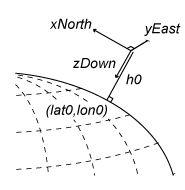
\includegraphics[scale=1]{figures/ned_system.png}
    \caption{Układ współrzędnych North-East-Down (NED).}
    \label{fig:elip_uklad}
\end{figure}
Układ ten budowany jest „w locie” i opiera się na umieszczeniu płaszczyzny stycznej do kuli ziemskiej dokładnie w punkcie, w którym znajduje się baza operacyjna statku ($X=0, Y=0, Z=0$). Osie układu definiuje się następująco:
\begin{itemize}
    \item Oś $X$ (\textit{North}) skierowana jest idealnie wzdłuż lokalnego południka geograficznego na północ geograficzną.
    \item Oś $Y$ (\textit{East}) skierowana jest wzdłuż lokalnego równoleżnika na wschód geograficzny.
    \item Oś $Z$ (\textit{Down}) skierowana jest ortogonalnie w dół (w stronę środka masy Ziemi), domykając prawoskrętny układ współrzędnych. Wynika z tego, że ujemne wartości na osi Z będą oznaczać wzrost wysokości statku nad ziemią (pułap $H_{alt} = -Z_{ned}$).
\end{itemize}

% -------------------------------------------------------

\subsection{Przykład praktyczny: Translacje za pomocą przybliżenia sferycznego}
Przy założeniu relatywnie krótkich misji (poniżej $10$ km długości wektora), krzywiznę elipsoidy w procedurach inżynierskich drona można zminimalizować do promienia kuli $R = 6\,378\,137$ m, co pozwala zredukować skomplikowane przekształcenia tensorowe Gaussa do bardzo prostego układu trygonometrycznego.

W niniejszym kursie algorytmika Pythona używa matematycznego wzoru do natychmiastowego przetłumaczenia zadanego przesunięcia w płaskim układzie kartezjańskim (np. "przesuń cel o $\Delta North$ oraz $\Delta East$ metrów") z powrotem na język globalnego modułu satelitarnego WGS84:

\begin{lstlisting}[language=Python, caption=Przeliczanie przesunięcia metrycznego w układzie NED na współrzędne GPS (w oparciu o promień kuli)]
def get_location_meters(original_location, d_north, d_east):
    earth_radius = 6378137.0
    
    # Krok 1: Wyliczenie offsetu katowego (w radianach)
    d_lat = d_north / earth_radius
    
    # Wspolrzedna East wymaga doliczenia funkcji 'cos', poniewaz obwody 
    # rownoleznikow zawezaja sie wraz ze zblizaniem sie do biebunow Ziemi
    d_lon = d_east / (earth_radius * math.cos(math.pi * original_location.lat / 180.0))
    
    # Krok 2: Zamiana radianow na stopnie dziesietne (decimal degrees)
    new_lat = original_location.lat + (d_lat * 180.0 / math.pi)
    new_lon = original_location.lon + (d_lon * 180.0 / math.pi)
    
    return LocationGlobalRelative(new_lat, new_lon, original_location.alt)
\end{lstlisting}

Podobne uproszczenia (przybliżenie Płaskiej Ziemi) stosujemy, obliczając najkrótszą odległość euklidesową (w metrach) pomiędzy dwoma punktami GPS. Znając z geometrii definicję miary Pitagorasa $\Delta d = \sqrt{\Delta x^2 + \Delta y^2}$, musimy jedynie odpowiednio wylistować długości łuków, korzystając ze stałego przelicznika $1^\circ \approx 111,319.5$ metrów. 
\begin{lstlisting}[language=Python, caption=Wyznaczanie odległości euklidesowej z układu geodezyjnego]
def get_distance_metres(loc1, loc2):
    """
    Krotki algorytm obliczania odleglosci euklidesowej w metrach. 
    Wzor wykorzystuje stala zamiane stopni na metry.
    """
    d_lat = loc2.lat - loc1.lat
    d_lon = loc2.lon - loc1.lon
    return math.sqrt((d_lat**2) + (d_lon**2)) * 1.113195e5
\end{lstlisting}
Tak przedstawiona dualność opisu trajektorii pozwala algorytmice drona realizować misje na geometrycznie doskonałej, dwuwymiarowej tablicy kartezjańskiej (co wybitnie sprawdza się m.in. w implementacji algorytmów Sweep-Line i Kosiarki z modułu CPP), jednocześnie gwarantując wykonanie poprawnego, wolnego od dryfu satelitarnego toru przelotu w świecie rzeczywistym.




\section{Krzywe parametryczne w modelowaniu trajektorii}

W klasycznym podejściu nawigacyjnym trajektorię lotu definiuje się jako uporządkowany ciąg punktów orientacyjnych (ang. \textit{waypoints}) $W = \{w_1, w_2, \dots, w_m\} \subset \mathbb{R}^3$, połączonych odcinkami prostoliniowymi. Choć metoda ta sprawdza się w misjach transportowych na dużych wysokościach, posiada fundamentalne wady w sterowaniu autonomicznym:
\begin{itemize}
    \item \textbf{Brak gładkości ($C^0$):} W węzłach $w_i$ wektor prędkości doznaje skokowej zmiany kierunku. Realizacja takiego ruchu przez układ fizyczny wymagałaby nieskończenie dużych sił (przyspieszeń), co w praktyce wymusza wyhamowanie statku niemal do zera przed każdym zakrętem.
    \item \textbf{Nieoptymalne zużycie energii:} Ciągłe cykle hamowania i przyspieszania drastycznie skracają czas pracy akumulatorów LiPo.
\end{itemize}

Rozwiązaniem tego problemu jest modelowanie toru ruchu za pomocą \textbf{krzywych parametrycznych klasy co najmniej $C^2$} (dwukrotnie różniczkowalnych w sposób ciągły):
\begin{equation}
    \mathbf{r}(t) = \begin{bmatrix} x(t) \\ y(t) \\ z(t) \end{bmatrix}, \quad t \in [t_0, t_k]
\end{equation}
gdzie parametr $t$ utożsamiamy najczęściej z czasem fizycznym. Taki opis pozwala na bezpośrednie wyznaczenie wektora prędkości $\mathbf{v}(t) = \mathbf{\dot{r}}(t)$ oraz wektora przyspieszenia $\mathbf{a}(t) = \mathbf{\ddot{r}}(t)$, co umożliwia kontrolerom lotu płynne sterowanie ciągiem i kątami przechylenia statku.


\subsection{Krzywe w przestrzeni 2D}

Rozważmy ruch w płaszczyźnie poziomej przy założeniu stałego pułapu ($z(t) = \text{const}$, $v_z = 0$). Niech $\mathbf{r}(t) = [x(t), y(t)]^T$ będzie krzywą płaską. 

\subsubsection{Krzywizna a ograniczenia fizyczne}
Kluczowym pojęciem analizy trajektorii jest jej \textbf{krzywizna} $\kappa(t)$, mierząca tempo zmiany kierunku wektora stycznego:
\begin{equation}
    \kappa(t) = \frac{|\dot{x}\ddot{y} - \dot{y}\ddot{x}|}{(\dot{x}^2 + \dot{y}^2)^{3/2}} = \frac{\|\mathbf{\dot{r}}(t) \times \mathbf{\ddot{r}}(t)\|}{\|\mathbf{\dot{r}}(t)\|^3}
\end{equation}
Z mechaniki newtonowskiej wynika, że ruch po krzywej o krzywiźnie $\kappa(t)$ z prędkością skalarną $v(t) = \|\mathbf{\dot{r}}(t)\|$ generuje przyspieszenie dośrodkowe:
\begin{equation}
    a_n(t) = v^2(t) \cdot \kappa(t)
\end{equation}
Ponieważ maksymalny kąt przechylenia drona (ang. \textit{tilt angle}) jest ograniczony parametrami konstrukcyjnymi i stabilnością aerodynamiczną, maksymalne dopuszczalne przyspieszenie boczne wynosi $a_{\max} = g \tan(\theta_{\max})$. Wprowadza to twarde ograniczenie na prędkość w zakręcie:
\begin{equation}
    v(t) \le \sqrt{\frac{a_{\max}}{\kappa(t)}}
\end{equation}
W punktach o dużej krzywiźnie $\kappa$ (ostre skręty) dron musi zredukować prędkość, natomiast na odcinkach o $\kappa \approx 0$ może poruszać się z prędkością maksymalną.

\subsubsection{Przykłady krzywych analitycznych}

W module \texttt{02\_fizyka\_i\_matematyka} (skrypt \texttt{03\_parametric\_shapes.py}) zaimplementowano trzy reprezentatywne geometrie:

\paragraph{1. Okrąg (Krzywa o stałej krzywiźnie):}
Najprostsza krzywa zamknięta o stałej krzywiźnie $\kappa = \frac{1}{R}$:
\begin{equation}
    \begin{cases}
        x(t) = R \cos(\omega t) - R \\
        y(t) = R \sin(\omega t)
    \end{cases}, \quad t \in \left[0, \frac{2\pi}{\omega}\right]
\end{equation}
Przesunięcie o $-R$ na osi $x$ zostało zastosowane w celu zapewnienia warunku początkowego $\mathbf{r}(0) = [0, 0]^T$, dzięki czemu dron rozpoczyna manewr bezpośrednio z punktu zawisu. Prędkość i przyspieszenie wynoszą odpowiednio:
\begin{align}
    \mathbf{v}(t) &= [-R\omega \sin(\omega t), R\omega \cos(\omega t)]^T, \quad \|\mathbf{v}(t)\| = R\omega = \text{const} \\
    \mathbf{a}(t) &= [-R\omega^2 \cos(\omega t), -R\omega^2 \sin(\omega t)]^T, \quad \|\mathbf{a}(t)\| = R\omega^2 = \text{const}
\end{align}
Stałość modułu przyspieszenia oznacza, że dron utrzymuje stały kąt przechyłu (Roll) przez cały czas trwania manewru.

\paragraph{2. Lemniskata Gerono (Ósemka):}
Krzywa w kształcie cyfry 8, stosowana powszechnie w procedurach kalibracji magnetometru (kompasu) BSP:
\begin{equation}
    \begin{cases}
        x(t) = A \sin(\omega t) \\
        y(t) = A \sin(\omega t)\cos(\omega t) = \frac{A}{2} \sin(2\omega t)
    \end{cases}, \quad t \in \left[0, \frac{2\pi}{\omega}\right]
\end{equation}
Krzywizna lemniskaty zmienia znak przy przejściu przez punkt węzłowy $(0,0)$, co wymaga od kontrolera lotu płynnego przejścia z przechyłu w lewo do przechyłu w prawo (inwersja wektora siły dośrodkowej).

\paragraph{3. Kardioida (Krzywa o zmiennej dynamice):}
Krzywa o równaniu wykorzystującym sumę harmonicznych, generująca kształt serca:
\begin{equation}
    \begin{cases}
        x(t) = 16A \sin^3(\omega t) \\
        y(t) = A \big(13\cos(\omega t) - 5\cos(2\omega t) - 2\cos(3\omega t) - \cos(4\omega t)\big)
    \end{cases}
\end{equation}
Trajektoria ta posiada ostrze (punkt osobliwy, w którym $\mathbf{\dot{r}}(t) \to 0$ przy zbliżaniu się do szpica), co stanowi doskonały poligon testowy dla algorytmów sprawdzających zachowanie pętli sterowania przy gwałtownych zmianach zwrotu wektora prędkości.

\subsubsection{Dyskretyzacja i filtracja geometryczna w kodzie}
Komputer pokładowy drona operuje w czasie dyskretnym z częstotliwością $f = \frac{1}{\Delta t}$. Ciągła krzywa $\mathbf{r}(t)$ jest próbkowana do postaci zbioru punktów węzłowych $\mathbf{P}_k = \mathbf{r}(k \Delta t)$ dla $k = 0, 1, \dots, N$. 

W skrypcie \texttt{03\_parametric\_shapes.py} zaimplementowano \textbf{pętlę nadążną z tolerancją promienia akceptacji} $r_{\text{tol}}$:
\begin{equation}
    \|\mathbf{r}_{\text{drone}} - \mathbf{P}_k\| \le r_{\text{tol}} \implies k \leftarrow k + 1
\end{equation}
Ustawienie $r_{\text{tol}} \approx 2.0\text{ m}$ działa jak mechaniczny filtr dolnoprzepustowy. Autopilot przełącza cel na kolejny punkt zanim statek zbiegnie do punktu bieżącego. Wykorzystuje to bezwładność drona do naturalnego zaokrąglania krzywej, eliminując szarpnięcia bez konieczności obliczania złożonych wielomianów wyższych rzędów na pokładzie mikrokontrolera.


\subsection{Krzywe w przestrzeni 3D}

W trójwymiarowej przestrzeni euklidesowej $\mathbb{R}^3$ trajektoria zyskuje dodatkowy stopień swobody: zmianę wysokości w czasie ($z(t)$). Z punktu widzenia geometrii różniczkowej, krzywą przestrzenną charakteryzują dwie wielkości lokalne: \textbf{krzywizna} $\kappa(t)$ oraz \textbf{skręcenie (torsja)} $\tau(t)$, opisujące zachowanie reperu Freneta-Serreta $(\mathbf{T}, \mathbf{N}, \mathbf{B})$:
\begin{equation}
    \frac{d\mathbf{T}}{ds} = \kappa \mathbf{N}, \quad 
    \frac{d\mathbf{N}}{ds} = -\kappa \mathbf{T} + \tau \mathbf{B}, \quad 
    \frac{d\mathbf{B}}{ds} = -\tau \mathbf{N}
\end{equation}
gdzie $s$ oznacza naturalny parametr długości łuku, $\mathbf{T}$ wektor styczny, $\mathbf{N}$ normalny, a $\mathbf{B} = \mathbf{T} \times \mathbf{N}$ binormalny. Torsja $\tau(t)$ określa tempo, z jakim krzywa "ucieka" z płaszczyzny ściśle stycznej.

\subsubsection{Helisa walcowa (Cylindrical Helix)}
Najprostsza trójwymiarowa krzywa przestrzenna o stałej krzywiźnie i stałym skręceniu. Powstaje przez nałożenie jednostajnego ruchu postępowego wzdłuż osi $z$ na ruch po okręgu:
\begin{equation}
    \mathbf{r}(t) = \begin{bmatrix} R \cos(\omega t) \\ R \sin(\omega t) \\ v_z \cdot t \end{bmatrix}, \quad t \ge 0
\end{equation}
Własności różniczkowe helisy walcowej wyrażają się wzorami:
\begin{equation}
    \kappa = \frac{R}{R^2 + (v_z/\omega)^2} = \text{const}, \quad \tau = \frac{v_z/\omega}{R^2 + (v_z/\omega)^2} = \text{const}
\end{equation}
Krzywa ta jest podstawowym wzorcem wykorzystywanym przy inspekcjach obiektów pionowych o przekroju kołowym (kominy, wieże telekomunikacyjne, turbiny wiatrowe).

\subsubsection{Helisa stożkowa (Conical Helix) -- Lejek poszukiwawczy}
W misjach poszukiwawczo-ratowniczych (SAR -- \textit{Search and Rescue}) stosuje się trajektorię o zmiennym promieniu i malejącej wysokości. Dron rozpoczyna przeszukiwanie na wysokim pułapie, zataczając szerokie kręgi w celu wykrycia sygnału z nadajnika ratunkowego, a następnie zawęża promień w miarę obniżania lotu, koncentrując się na źródle sygnału.

Równanie parametryczne helisy stożkowej ma postać:
\begin{equation}
    \begin{cases}
        x(t) = R(t) \cos(\omega t) \\
        y(t) = R(t) \sin(\omega t) \\
        z(t) = Z_0 - v_z \cdot t
    \end{cases}
\end{equation}
gdzie promień maleje liniowo wraz z upływem czasu:
\begin{equation}
    R(t) = R_0 \left(1 - \alpha \frac{t}{t_k}\right), \quad \alpha \in (0, 1)
\end{equation}
Kinematyka tego ruchu wymaga od sterownika jednoczesnej modulacji prędkości we wszystkich trzech osiach. Różniczkując wektor położenia po czasie otrzymujemy wektor prędkości zadanej:
\begin{equation}
    \mathbf{v}(t) = \mathbf{\dot{r}}(t) = \begin{bmatrix}
        \dot{R}(t)\cos(\omega t) - R(t)\omega\sin(\omega t) \\
        \dot{R}(t)\sin(\omega t) + R(t)\omega\cos(\omega t) \\
        -v_z
    \end{bmatrix}
\end{equation}
gdzie $\dot{R}(t) = -\frac{\alpha R_0}{t_k} = \text{const}$. 

\subsubsection{Trajektorie na powierzchniach walcowych (Inspekcja 3D)}
W zaawansowanych misjach fotogrametrycznych (patrz skrypt \texttt{07\_c\_cylinder\_scan.py}) trajektorię generuje się nie w przestrzeni swobodnej, lecz w oparciu o geometrię badanego obiektu. 

Jeżeli środek obiektu znajduje się w punkcie geograficznym $\mathbf{P}_{\text{target}} = (\text{lat}_0, \text{lon}_0)$, a jego wysokość wynosi $H_{\text{bld}}$, wówczas trajektorię definiuje się we współrzędnych walcowych $(r, \theta, z)$ sprowadzonych do bazy NED:
\begin{equation}
    \mathbf{r}_{\text{NED}}(\theta, z) = \begin{bmatrix}
        N_{\text{target}} + R_{\text{scan}} \cos(\theta) \\
        E_{\text{target}} + R_{\text{scan}} \sin(\theta) \\
        -z
    \end{bmatrix}, \quad \theta \in [0, 2\pi], \; z \in [Z_{\min}, Z_{\max}]
\end{equation}
Skanowanie realizowane jest poprzez dyskretne warstwy wysokościowe $z_k \in \{h_1, h_2, \dots, h_m\}$ (orbity poziome na stałych wysokościach) lub w postaci pionowego meandra (ang. \textit{raster path}), w którym dron przemieszcza się naprzemiennie w górę i w dół, dokonując obrotu o stały kąt $\Delta\theta$ na szczycie i u podstawy cylindra. Zapewnia to stałą odległość kamery od elewacji, co jest warunkiem koniecznym do uzyskania stałej rozdzielczości terenowej zdjęć (GSD -- \textit{Ground Sample Distance}).


\section{Równania różniczkowe zwyczajne (ODE) w kinematyce}

Zrozumienie działania algorytmów nawigacyjnych, kontrolerów lotu oraz metod synchronizacji systemów wieloagentowych (np. lotu w roju) wymaga odwołania się do podstaw rachunku różniczkowego. W fizyce klasycznej i robotyce stan obiektu opisuje się wektorem jego położeń $\mathbf{x}(t) \in \mathbb{R}^d$ oraz prędkości $\mathbf{v}(t) = \mathbf{x}'(t) \in \mathbb{R}^d$. Ze względu na drugą zasadę dynamiki Newtona ($F = ma$), układy mechaniczne modeluje się najczęściej za pomocą równań różniczkowych zwyczajnych drugiego rzędu (wiążących przyspieszenie $\mathbf{x}''(t)$ ze stanem układu).

\subsection{Zagadnienie początkowe Cauchy'ego dla układów autonomicznych}

W analizie ruchu dronów najczęściej rozważamy modele niezależne bezpośrednio od upływu czasu (tzw. układy autonomiczne), gdzie ewolucja zależy wyłącznie od bieżącego położenia i prędkości w przestrzeni. Równanie ruchu zapisujemy w ogólnej postaci:
\begin{equation}
    \mathbf{x}'' = f(\mathbf{x}, \mathbf{x}')
\end{equation}
Aby z równania różniczkowego móc wyznaczyć jedną, konkretną trajektorię fizyczną spośród nieskończonej rodziny rozwiązań, konieczne jest sformułowanie tzw. \textbf{zagadnienia początkowego Cauchy'ego}. Polega ono na podaniu warunków początkowych, czyli stanu wektora w wybranej chwili $t_0 = 0$:
\begin{equation}
    \begin{cases}
        \mathbf{x}'' = f(\mathbf{x}, \mathbf{x}') \\
        \mathbf{x}(0) = \mathbf{x}_0 \\
        \mathbf{x}'(0) = \mathbf{v}_0
    \end{cases}
    \label{eq:cauchy_ivp}
\end{equation}
Równanie to jest rozwiązywane w locie (przez sprzętowy kontroler lotu) – dla zadanego stanu $(x_0, v_0)$ komputer oblicza przyspieszenie i całkuje je w przód, by określić stan drona ułamek sekundy później.

\subsubsection{Wpływ składników funkcji wymuszającej $f(\mathbf{x}, \mathbf{x}')$}
Zależność funkcji przyspieszenia od poszczególnych pochodnych warunkuje charakter dynamiki układu:
\begin{itemize}
    \item \textbf{Brak zależności od $\mathbf{x}'$ ($f = f(\mathbf{x})$):} Układ jest \textit{zachowawczy}. Siła zależy wyłącznie od geometrii otoczenia. Klasycznym przykładem jest pole grawitacyjne ($\mathbf{x}'' = \mathbf{g}$) lub nieliniowy oscylator harmoniczny (np. wahadło bez oporów: $x'' = -\sin x$). Energia mechaniczna takiego systemu jest stała. Brak zależności od prędkości oznacza, że dron sterowany takim algorytmem nigdy nie wyhamuje – będzie oscylował w nieskończoność wokół punktu docelowego.
    \item \textbf{Zależność od $\mathbf{x}'$ ($f = f(\mathbf{x}, \mathbf{x}')$):} Wprowadza do układu dyssypację (rozpraszanie energii) lub aktywne napędzanie. Składniki ujemnie proporcjonalne do prędkości (np. $-c \mathbf{x}'$) modelują siły oporu aerodynamicznego drona. Z punktu widzenia automatyki (regulatorów PD), wprowadzenie zależności od pochodnej błędu pozwala na wytłumienie oscylacji i stabilne zatrzymanie drona w punkcie docelowym. W algorytmach roju to właśnie zależność od $\mathbf{x}'$ sąsiada decyduje o synchronizacji (zrównaniu prędkości).
\end{itemize}


\subsection{Zagadnienia brzegowe w optymalizacji trajektorii}

W opozycji do zagadnienia początkowego (gdzie znamy "Start" i prognozujemy przyszłość), w problemach planowania autonomicznych misji (np. precyzyjnego omijania przeszkód przy dojeściu do celu) znacznie częściej formułuje się \textbf{zagadnienie brzegowe} (ang. \textit{Boundary Value Problem -- BVP}).

W układzie drugiego rzędu przyjmuje ono postać:
\begin{equation}
    \begin{cases}
        F(\mathbf{x}, \mathbf{x}', \mathbf{x}'') = 0 \\
        B_1(\mathbf{x}(t_0), \mathbf{x}'(t_0)) = \alpha \\
        B_2(\mathbf{x}(t_k), \mathbf{x}'(t_k)) = \beta
    \end{cases}
\end{equation}
Oznacza to, że znamy stan w chwili początkowej $t_0$ (np. start z bazy) oraz pożądany stan w zadanej chwili końcowej $t_k$ (np. dron musi dotrzeć do strefy zrzutu ze zredukowaną prędkością). Poszukujemy takiej trajektorii $\mathbf{x}(t)$, która przejdzie przez te konkretne dwa stany graniczne, minimalizując często dodatkowy funkcjonał kosztu (np. najmniejsze zużycie energii $\int (\mathbf{x}'')^2 dt$). Rozwiązanie analityczne zagadnień brzegowych jest zazwyczaj niemożliwe, dlatego wykorzystuje się zaawansowane algorytmy numeryczne (tzw. \textit{Shooting Methods} lub \textit{Collocation Methods}).


\subsection{Zastosowanie na przykładzie: Model Cuckera-Smale'a}

Doskonałym przykładem pokazującym jak abstrakcyjne równania różniczkowe kontrolują rzeczywistą, fizyczną chmarę statków powietrznych, jest \textbf{model Cuckera-Smale’a (C-S)}\footnote{Cucker, F., Smale, S., \textit{Emergent Behavior in Flocks}, IEEE Transactions on Automatic Control, 2007.}. Jest to nieliniowy układ równań różniczkowych zwyczajnych drugiego rzędu, opisujący zjawisko tzw. \textit{flockingu} (gromadnego lotu, np. klucza ptaków).

Niech $N$ oznacza liczbę dronów w roju. Dla $i$-tego drona jego pozycja to $\mathbf{x}_i \in \mathbb{R}^3$, a prędkość to $\mathbf{v}_i = \mathbf{x}'_i$. Klasyczny układ równań C-S (dla $i=1,\dots,N$) ma postać:
\begin{equation}
    \begin{cases}
        \mathbf{x}'_i = \mathbf{v}_i \\
        \mathbf{v}'_i = \frac{K}{N} \sum_{j=1}^{N} \psi(\|\mathbf{x}_j - \mathbf{x}_i\|) \cdot (\mathbf{v}_j - \mathbf{v}_i)
    \end{cases}
    \label{eq:cs_original}
\end{equation}
gdzie funkcja wagi $\psi(r)$ (tzw. potencjał oddziaływania) określa jak bardzo dystans osłabia chęć synchronizacji:
\begin{equation}
    \psi(r) = \frac{1}{(1 + r^2)^\beta}, \quad \beta \ge 0
\end{equation}

\subsubsection{Analiza matematyczna i zbieżność}
Równanie \eqref{eq:cs_original} oznacza, że przyspieszenie ($\mathbf{v}'_i$) drona opiera się wyłącznie na \textbf{różnicy prędkości} między nim a sąsiadami ($\mathbf{v}_j - \mathbf{v}_i$). 
Fundamentalne twierdzenie Cuckera i Smale'a dowodzi asymtotycznego powstania konsensusu (zjawiska \textit{flockingu}): Jeśli $\beta < \frac{1}{2}$, to dla dowolnych warunków początkowych (niezależnie jak drony są na starcie rozproszone), w granicy $t \to \infty$ prędkości wszystkich dronów zbiegają się do wspólnego wektora prędkości średniej $\bar{\mathbf{v}}$, a dystans między każdą parą zbiega do stałej wartości. Rój leci w idealnym szyku.

\subsubsection{Modyfikacje hybrydowe do zastosowań inżynierskich}
W implementacji informatycznej (skrypt \texttt{05\_a\_cucker\_smale\_model.py}) czysty system ODE został rozbudowany o dwa krytyczne człony nieliniowe (dodatkowe funkcje wymuszające), aby sprostać wymaganiom bezpieczeństwa przestrzeni powietrznej:

\begin{enumerate}
    \item \textbf{Potencjał Repulsyjny (Antykolizja):} 
    Oryginalny system \eqref{eq:cs_original} nie zabrania pokrycia się dwóch obiektów w punkcie ($\mathbf{x}_i = \mathbf{x}_j$). Wprowadzono siłę odpychającą działającą na zasadzie odwrotnych sześcianów, która aktywuje się tylko w strefie niebezpiecznej ($r < D_{\text{safe}}$):
    \begin{equation}
        \mathbf{F}_{\text{rep}, i} = R \sum_{j \ne i, \|\mathbf{x}_{ij}\| < D_{\text{safe}}} \frac{\mathbf{x}_i - \mathbf{x}_j}{\|\mathbf{x}_i - \mathbf{x}_j\|^3}
    \end{equation}
    gdzie $R$ to stała siły odpychania. Zależność od samego położenia ($\mathbf{x}$) działa tu jak sztywna, nieliniowa sprężyna mechaniczna.
    
    \item \textbf{Zależność Leader-Follower (Kohezja kierunkowa):}
    W systemach z podziałem decyzyjnym wyznacza się jednego agenta (Lidera, $i=0$), którego dynamika jest niezależna od układu (np. realizuje zewnętrzną misję zagadnienia brzegowego). Pozostałe drony $i \in \{1,\dots,N-1\}$ zostają poddane dodatkowemu przyciąganiu do Lidera na wzór oscylatora tłumionego (gdzie rolę tłumienia pełni mechanizm Cuckera-Smale'a):
    \begin{equation}
        \mathbf{F}_{\text{coh}, i} = K_{\text{coh}} (\mathbf{x}_0 - \mathbf{x}_i)
    \end{equation}
\end{enumerate}

Ostateczny kształt hybrydowego równania różniczkowego ruchu dyskretnie całkowanego przez nasz skrypt na pokładzie roju przyjmuje postać silnie nieliniowego równania 2-go rzędu:
\begin{equation}
    \mathbf{v}'_i = \underbrace{ K_{\text{cs}} \sum_{j} \frac{\mathbf{v}_j - \mathbf{v}_i}{(1 + \|\mathbf{x}_{ij}\|^2)^\beta} }_{\text{Synchronizacja (C-S)}} 
    + \underbrace{ R \sum_{j} \frac{\mathbf{x}_{ij}}{\|\mathbf{x}_{ij}\|^3} }_{\text{Repulsja}} 
    + \underbrace{ K_{\text{coh}} (\mathbf{x}_0 - \mathbf{x}_i) }_{\text{Kohezja do Lidera}}
\end{equation}
Tak zdefiniowany system gwarantuje nie tylko samoczynne formowanie się klastrów o wspólnej prędkości, ale również odporność na turbulencje oraz brak kolizji fizycznych w przestrzeni trójwymiarowej.


\section{Numeryczne całkowanie równań ruchu}
Ze względu na brak ciągłości czasu w układach mikroprocesorowych, pochodne zastępowane są ilorazami różnicowymi dla dyskretnego kroku czasowego $\Delta t$. Wybór metody całkowania jest zawsze kompromisem pomiędzy złożonością obliczeniową (obciążeniem procesora) a stabilnością (dokładnością fizyki).

\subsection{Metoda Eulera (rzędu pierwszego)}
Najprostszą formą rozwiązywania zagadnień początkowych jest jawna metoda Eulera. W każdym kroku pętli zakłada ona, że pochodna (np. prędkość) jest stała na przestrzeni interwału $\Delta t$:
\begin{align}
    \vec{v}_{n+1} &= \vec{v}_n + \vec{a}(\vec{x}_n, \vec{v}_n, t_n) \cdot \Delta t \\
    \vec{x}_{n+1} &= \vec{x}_n + \vec{v}_n \cdot \Delta t
\end{align}

Wadą tej metody jest szybka akumulacja błędu globalnego (wynoszącego $\mathcal{O}(\Delta t)$), co w symulacji lotu prowadzi do powolnego "rozjeżdżania się" estymowanego położenia z rzeczywistością, jeśli krok $\Delta t$ jest zbyt duży. Jest ona jednak powszechnie stosowana w skryptach wysokiego poziomu (np. naszych algorytmach Cuckera-Smale'a) ze względu na łatwość implementacji oraz dominujący wpływ zewnętrznych układów stabilizujących (PID drona koryguje nasze błędy numeryczne).

\subsection{Metoda Rungego-Kutty (rzędu czwartego - RK4)}
Standardem w silnikach fizycznych symulatorów (takich jak wewnętrzny model SITL) są wielokrokowe metody wyższego rzędu, głównie algorytm RK4. Aby obliczyć nowe położenie, metoda RK4 probkuje pochodną funkcji w czterech punktach wewnątrz kroku $\Delta t$ (na początku, dwukrotnie w połowie i na końcu przedziału), po czym uśrednia te wektory z odpowiednimi wagami.
Skutkuje to redukcją błędu rzędu $\mathcal{O}(\Delta t^4)$, co zapewnia niezbędną, absolutną stabilność numeryczną przy odtwarzaniu agresywnych manewrów aerodynamicznych drona, unikając jednoczesnego zjawiska numerycznej eksplozji układu.
\chapter{Fizyczne podstawy}
% =======================================================
\section{Dynamika bryły sztywnej w 6 stopniach swobody (6-DOF)}
% Teoria: Masa, inercja, środek ciężkości. Kąty Eulera: Roll (Przechył), Pitch (Pochylenie), Yaw (Odchylenie). Jak wektor ciągu silników wpływa na ruch w konkretnym kierunku.

\section{Zakłócenia zewnętrzne i estymacja stanu}
% Teoria: Szum czujników (GPS, barometr, IMU). Dlaczego pomiary nigdy nie są idealne?
\subsection{Zjawisko znoszenia (Wind drift) i Rozszerzony Filtr Kalmana (EKF)}
% Teoria: Fuzja sensorów. Jak dron domyśla się obecności wiatru analizując różnicę między modelem matematycznym a faktycznym przesunięciem GPS.
\subsection{Przykład praktyczny: Nasłuchiwanie telemetrii w warunkach silnego wiatru}
% Kod Python: Skrypt 04_physics_wind.py. Odczyt danych z MAVLinka i analiza kompensacji wektora wiatru.


% =======================================================
\chapter{Programistyczne podstawy}
% =======================================================

Kiedy aparat matematyczny określi pożądaną trajektorię lotu, a modele fizyczne zweryfikują jej wykonalność, niezbędne jest przeniesienie tego abstrakcyjnego opisu na fizyczną maszynę. W tym rozdziale omówiona zostanie architektura nowoczesnych systemów bezzałogowych, protokoły komunikacyjne oraz paradygmaty programistyczne pozwalające na tworzenie wysoce niezawodnego oprogramowania kontrolującego BSP w czasie rzeczywistym.

\section{Architektura systemów bezzałogowych (Hardware i Software)}

Aby bezpiecznie realizować misje autonomiczne, współczesne drony wykorzystują architekturę podzieloną na dwie niezależne warstwy obliczeniowe, co gwarantuje separację krytycznych systemów bezpieczeństwa (ang. \textit{Fault Tolerance}) od systemów decyzyjnych.

\begin{enumerate}
    \item \textbf{Autopilot (Kontroler Lotu -- Flight Controller):}
    Jest to niskopoziomowy układ scalony (mikrokontroler, np. STM32), na którym działa System Czasu Rzeczywistego (RTOS). Jego jedynym zadaniem jest czytanie sensorów z częstotliwością np. 400\,Hz, uruchamianie filtrów EKF i wyliczanie sygnałów PWM dla silników. Oprogramowanie to (np. ArduPilot) jest krytyczne dla życia statku. Autopilot nie „myśli” o skomplikowanych algorytmach optymalizacyjnych czy przetwarzaniu obrazu – po prostu zapewnia, by maszyna utrzymała się w powietrzu.

    \item \textbf{Komputer Pokładowy (Companion Computer):}
    Jest to wysokopoziomowy mikrokomputer (np. Raspberry Pi, Nvidia Jetson) działający na systemie operacyjnym klasy Linux. Uruchamiany jest na nim kod w języku Python lub C++ (np. nasze skrypty z kursu). Komputer pokładowy przetwarza trudne matematycznie algorytmy (TSP, nawigacja predykcyjna) i za pomocą kabla szeregowego podaje Autopilotowi proste komendy, np. \textit{„leć prosto z prędkością 5 m/s”}. W razie awarii (zawieszenia się) Komputera Pokładowego, Autopilot nadal działa i może bezpiecznie wylądować statkiem.
\end{enumerate}

\section{Symulator SITL i protokół MAVLink}

Nauka i testowanie algorytmów nawigacyjnych na fizycznych dronach jest niepraktyczna, ryzykowna i niezwykle kosztowna. Z tego powodu inżynieria lotnicza stosuje podejście \textbf{Software-In-The-Loop (SITL)}.

W symulacji SITL ten sam skompilowany kod (w C++), który trafiłby na fizyczny procesor Autopilota, uruchamiany jest jako izolowany proces w systemie Linux. Silnik fizyczny w tle oszukuje to oprogramowanie, wysyłając do niego sztuczne pomiary z wirtualnego GPS-u, wiatromierza i barometru. Dzięki temu testowany skrypt Pythona "nie wie", że rozmawia z programem na komputerze – jest to środowisko o niemal 100\% wierności w stosunku do lotu w świecie rzeczywistym.

\subsection{Protokół komunikacyjny MAVLink}

Wymiana informacji między Komputerem Pokładowym (Python) a Autopilotem (SITL) odbywa się w warstwie sieciowej (zwykle po portach UDP/TCP) przy użyciu \textbf{Protokołu MAVLink} (\textit{Micro Air Vehicle Link}). 
MAVLink to wysoce odchudzony, binarny protokół komunikacyjny. Każda wiadomość (np. odczyt wysokości lub komenda ruchu) pakowana jest w kilkunastobajtową ramkę danych, co zapewnia szybkość transmisji i odporność na utratę pakietów w sieciach bezprzewodowych.

W naszej architekturze rolę centralnego routera odgrywa program \textbf{MAVProxy}. Łączy się on z symulatorem (Dronem) i dystrybuuje pakiety MAVLink na lokalne porty UDP (np. \texttt{127.0.0.1:14550}), do których następnie "podpinają się" nasze skrypty Pythona.

\subsection{Przykład praktyczny: Inicjalizacja środowiska}

W kursie wykorzystujemy skrypty w powłoce \texttt{Bash}, które automatyzują proces uruchamiania infrastruktury sieciowej dla SITL.
\begin{lstlisting}[language=bash, caption=Skrypt startowy powołujący wirtualnego drona do życia]
#!/bin/bash
# Zmienne srodowiskowe wczytywane z .profile zapewniaja dostep do narzedzi ArduPilota
source ~/.profile

# Uruchomienie fizyki i routera w tle
# Flaga --map otwiera interfejs graficzny GCS, 
# a --out=127.0.0.1:14550 wyprowadza sygnal MAVLink dla naszego Pythona.
cd ~/ardupilot/ArduCopter
sim_vehicle.py -v ArduCopter -f + --map --out=127.0.0.1:14550
\end{lstlisting}


\section{Paradygmat asynchroniczny i tryby lotu}

Pisanie programów sterujących dla dronów różni się fundamentalnie od pisania klasycznych aplikacji sekwencyjnych. Prawa fizyki nakazują programiście dostosowanie się do \textbf{paradygmatu asynchronicznego} -- komenda wysłana z Pythona (np. \textit{„wystartuj na 10 metrów”}) wykonuje się w mikrosekundę w CPU, ale jej fizyczna realizacja przez maszyny elektryczne i śmigła trwa kilkanaście sekund.

Dlatego kod drona obfituje w \textbf{Maszyny Stanów (State Machines)} oraz niekończące się pętle (pętle nadążne), które upewniają się, że uwarunkowania fizyczne zostały spełnione przed przejściem do kolejnej instrukcji.

\subsection{Tryby lotu (Flight Modes)}
Stan i stopień autonomii decyzyjnej drona zależy od wymuszonego w MAVLinku trybu:
\begin{itemize}
    \item \textbf{STABILIZE:} Dron ignoruje wektory z komputera pokładowego, odpowiada jedynie na manualne wychylenia drążków z aparatury sterującej operatora.
    \item \textbf{GUIDED:} Tryb autonomii zewnętrznej. Autopilot dba o stabilizację wiatrową, ale to zewnętrzny skrypt Pythona ma pełną kontrolę na bieżąco, wysyłając mu ciągle nowe współrzędne docelowe lub wektory prędkości.
    \item \textbf{AUTO:} Tryb autonomii wewnętrznej. Dron całkowicie odcina się od zewnętrznych systemów sterowania na żywo i samodzielnie, punkt po punkcie, realizuje misję wyciągniętą ze swojej pamięci nieulotnej (EEPROM). Skrypt Pythona pełni tu jedynie funkcję obserwatora/nadzorcy.
    \item \textbf{RTL (Return To Launch):} Tryb awaryjny (z ang. powrót do startu). Wyzwolony z komputera lub automatycznie (tzw. Failsafe z powodu braku baterii), ignoruje wszelkie komendy, wznosi się na pułap bezpieczny i ląduje w bazie.
\end{itemize}

\subsection{Przykład praktyczny: Bezpieczna maszyna stanów}

Biblioteka \texttt{dronekit} dla języka Python stanowi wysokopoziomową otoczkę (ang. \textit{wrapper}) nad surowym protokołem MAVLink. Umożliwia ona manipulowanie stanem drona poprzez obiekty klas i ich atrybuty. Poniższy kod (fragment skryptu \texttt{01\_start.py}) demonstruje prawidłową obsługę asynchronicznych opóźnień:

\begin{lstlisting}[language=Python, caption=Procedura nawiązywania połączenia i bezpiecznego uzbrajania maszyny]
from dronekit import connect, VehicleMode
import time

def arm_and_takeoff(vehicle, target_altitude: float) -> None:
    # 1. Zabezpieczenie przed brakiem gotowosci (Pre-arm Checks).
    # vehicle.is_armable to dynamiczny atrybut, ktory zwraca True dopiero w momencie,
    # gdy wewnetrzne systemy EKF i GPS zglosza fizyczna gotowosc do lotu.
    print("Waiting for vehicle initialization...")
    while not vehicle.is_armable:
        time.sleep(1)
        
    # 2. Bezpieczna zmiana Trybu Lotu na GUIDED
    print("Setting mode to GUIDED and Arming motors...")
    vehicle.mode = VehicleMode("GUIDED")
    vehicle.armed = True # Wysłanie fizycznego odbezpieczenia śmigieł
    
    # 3. Asynchroniczne sprawdzenie (Silniki potrzebują ułamka sekundy na rozruch)
    while not vehicle.armed:
        time.sleep(1)
        
    print(f"Taking off to {target_altitude} meters...")
    vehicle.simple_takeoff(target_altitude)
    
    # 4. Pętla nadążna (Wznoszenie drona z uzyciem barometru/GPS)
    while True:
        # vehicle.location.global_relative_frame to zagnieżdżony obiekt (klasa LocationGlobalRelative),
        # którego atrybut '.alt' zwraca wysokość (w metrach) względem miejsca startu.
        current_altitude = vehicle.location.global_relative_frame.alt
        if current_altitude >= target_altitude * 0.95:
            # 95% tolerancji wynika z zasady nieoznaczoności w fizyce (błąd szumu czujników). 
            # Dron idealnie w cel nigdy nie trafi.
            print("Cruising altitude reached.")
            break
        time.sleep(1)
\end{lstlisting}


\section{Nawigacja punktowa a kontrola wektorowa}

W ramach biblioteki DroneKit oraz MAVLink istnieją dwa rozłączne paradygmaty przemieszczania drona w przestrzeni kosztem zużycia energii elektrycznej.

\subsection{Nawigacja punktowa (Position Control)}
Realizowana poprzez metody takie jak \texttt{vehicle.simple\_goto(target\_location)}. Jako wejście otrzymuje ściśle zdefiniowany punkt GPS. 
Paradygmat ten polega na przerzuceniu całej matematyki optymalizacyjnej na kontroler \textit{Autopilota}. To niskopoziomowe PID-y na płytce wyliczają, z jaką prędkością dron ma ruszyć i kiedy ma zacząć hamować. Podejście to jest niezawodne i szeroko opisane na przykładzie wyznaczania parametrycznych trajektorii w module matematycznym (np. kwadrat ze skryptu \texttt{02\_trajectory.py}).

\subsection{Kontrola wektorowa (Velocity Control)}
W przypadku zaawansowanych zagadnień takich jak unikanie kolizji (Repulsja), pościg w 3D czy algorytmy zachowań stadnych (Cucker-Smale), określenie docelowej współrzędnej nie jest fizycznie wykonalne – dążymy bowiem do zmiany \textbf{kierunku oraz prędkości} w danym, krótkim interwale $\Delta t$.

Realizuje to bezpośrednia ingerencja w wektor prędkości przy użyciu \textbf{surowych pakietów MAVLink}.
Wysłanie wiadomości o identyfikatorze \texttt{SET\_POSITION\_TARGET\_LOCAL\_NED} pozwala ominąć nawigatora Autopilota i wysłać żądane przyspieszenia bezpośrednio na układ aerodynamiczny.

\begin{lstlisting}[language=Python, caption=Wysyłanie bezpośredniego wektora prędkości do silników drona]
from pymavlink import mavutil

def send_ned_velocity(vehicle, velocity_x: float, velocity_y: float, velocity_z: float) -> None:
    """Wysyła wektor prędkości (m/s) w układzie NED."""
    # message_factory tworzy i pakuje strumień bitów zgodnie ze standardem MAVLink.
    msg = vehicle.message_factory.set_position_target_local_ned_encode(
        0, 0, 0, 
        mavutil.mavlink.MAV_FRAME_LOCAL_NED, # Definicja ukladu odniesienia (North, East, Down)
        0b0000111111000111, # Maska bitowa: nakazuje zignorowac pozycję, a wykonac TYLKO predkosc.
        0, 0, 0, # Parametry pozycji (ignorowane dzięki masce)
        velocity_x, velocity_y, velocity_z, # Zadane przez nas predkosci na 3 osiach w metrach/sekunde
        0, 0, 0, 0, 0 # Parametry przyspieszenia i yaw (ignorowane)
    )
    vehicle.send_mavlink(msg)
\end{lstlisting}

Podstawową cechą (i zagrożeniem) stosowania kontroli wektorowej jest fakt, że wektory wysyłane w ten sposób są natychmiastowe. Jeśli program w Pythonie przestanie z jakiegokolwiek powodu wysyłać w pętli nowe wektory, dron może kontynuować lot w zadanym wcześniej kierunku w nieskończoność. Dlatego algorytmy te wymagają najwyższej jakości kodu oraz ścisłego panowania nad synchronizacją czasu (`dt`).
% =======================================================
\chapter{Algorytmy ruchu indywidualnego w 3D}
% =======================================================

Przejście od nawigacji reaktywnej (sterowanie krok po kroku) do realizacji pełnych misji autonomicznych wymaga wykorzystania zaawansowanej algorytmiki i geometrii obliczeniowej. W tym rozdziale przedstawione zostaną trzy kanoniczne problemy robotyki mobilnej: planowanie pokrycia powierzchni (ang. \textit{Coverage Path Planning}), logistyczna optymalizacja trajektorii w grafach oraz przestrzenne przewidywanie ruchu obcych obiektów powietrznych.

\section{Geometria obliczeniowa w planowaniu misji (CPP)}

Problem Planowania Ścieżki Pokrycia (\textit{Coverage Path Planning} -- CPP) sprowadza się do znalezienia takiej trasy robota, która gwarantuje eksplorację zadanego obszaru $\mathcal{W}$ w całości, przy minimalizacji nadmiarowych przejść oraz zużycia energii. Zastosowanie CPP w lotnictwie bezzałogowym to przede wszystkim fotogrametria, rolnictwo precyzyjne (opryski) oraz operacje poszukiwawczo-ratownicze. Powszechnie stosowaną metodą rozwiązywania tego problemu jest klasyczny algorytm w kształcie meandra (wzór Boustrophedon / wzór Kosiarki).

\subsection{Algorytm zamiatania (Sweep-line) dla nieregularnych wielokątów}

Generowanie kosiarki dla idealnego, prostokątnego obszaru jest trywialne. Problem staje się obliczeniowo i analitycznie wymagający, gdy przestrzeń operacyjna $\mathcal{W}$ zadana jest jako dowolny wielokąt nieregularny, zdefiniowany przez uporządkowany zbiór wierzchołków $P = \{p_1, p_2, \dots, p_n\}$.

Aby ułożyć równoległe "paski" skanowania idealnie przycięte do obrysu pola (bez wylatywania drona poza wyznaczony teren, co marnowałoby cenną energię), stosuje się metodę \textbf{linii zamiatającej (ang. \textit{Sweep-line})}. 

\begin{figure}[ht]
    \centering
    \begin{tikzpicture}[scale=1.2]
        % Wielokąt (Poligon)
        \draw[thick, fill=green!10] (0, 0) -- (4, -1) -- (5, 3) -- (2, 4) -- (-1, 2) -- cycle;
        
        % Węzły wielokąta
        \filldraw (0,0) circle (1.5pt) node[below left] {$p_1$};
        \filldraw (4,-1) circle (1.5pt) node[below right] {$p_2$};
        \filldraw (5,3) circle (1.5pt) node[right] {$p_3$};
        \filldraw (2,4) circle (1.5pt) node[above] {$p_4$};
        \filldraw (-1,2) circle (1.5pt) node[left] {$p_5$};
        
        % Oś Sweep-Line
        \draw[->, >=stealth, thick, gray] (-2, -1.5) -- (-2, 4.5) node[above] {North ($N$)};
        \draw[->, >=stealth, thick, gray] (-2, -1.5) -- (5.5, -1.5) node[right] {East ($E$)};
        
        % Pojedyncza linia Sweep
        \draw[dashed, red, thick] (-1.5, 1.5) -- (5.5, 1.5) node[right] {$N = N_{\text{curr}}$};
        
        % Punkty przecięcia
        \filldraw[red] (-0.75, 1.5) circle (2pt) node[above left, text=black] {$I_1$};
        \filldraw[red] (4.62, 1.5) circle (2pt) node[above right, text=black] {$I_2$};
        
        % Zaznaczenie przecinanych odcinków
        \draw[blue, very thick] (-1,2) -- (0,0);
        \draw[blue, very thick] (4,-1) -- (5,3);
        
        % Trasa kosiarki (Boustrophedon)
        \draw[->, >=stealth, orange, line width=1.2pt] (-0.75, 1.5) -- (4.62, 1.5);
    \end{tikzpicture}
    \caption{Zasada działania algorytmu Sweep-Line. Pozioma prosta (czerwona przerywana) przecina boki wielokąta, wyznaczając granice ścieżki przelotu (pomarańczowa strzałka) dla drona na danej osi rzędnych.}
    \label{fig:sweepline}
\end{figure}

\subsubsection{Matematyka punktu przecięcia}
Rozważmy poziomą prostą przesuwającą się wzdłuż osi North o z góry ustaloną wartość kroku $w$ (ang. \textit{swath width} -- wynikającą z szerokości obiektywu kamery). Z definicji, prosta pozioma ma równanie $N = N_{\text{curr}}$. 

Weźmy dowolny bok wielokąta łączący punkty $p_a = (N_a, E_a)$ oraz $p_b = (N_b, E_b)$. Warunkiem koniecznym przecięcia tego boku przez naszą prostą jest, aby rzędna $N_{\text{curr}}$ znajdowała się pomiędzy wierzchołkami odcinka:
\begin{equation}
    (N_a \le N_{\text{curr}} < N_b) \quad \lor \quad (N_b \le N_{\text{curr}} < N_a)
\end{equation}
Gdy ten warunek jest spełniony, rozwiązujemy równanie prostej przechodzącej przez dwa punkty dla zmiennej $E_{\text{intersect}}$:
\begin{equation}
    E_{\text{intersect}} = E_a + (E_b - E_a) \frac{N_{\text{curr}} - N_a}{N_b - N_a}
\end{equation}

Dla prostego, wypukłego wielokąta, algorytm znajdzie zawsze dokładnie dwa punkty przecięcia dla każdej linii (lewy i prawy skraj), tworząc w ten sposób precyzyjne odległości, po których dron wykona przelot. Zobacz implementację w skrypcie \texttt{07\_a\_polygon\_scan.py}.

\subsubsection{Algorytm wyznaczania trasy (Pseudokod)}
\begin{enumerate}
    \item Wyznacz wierzchołki ekstremalne wielokąta dla Bounding Boxa: $N_{\min}$ oraz $N_{\max}$.
    \item Zainicjalizuj $N_{\text{curr}} = N_{\min} + \frac{w}{2}$ oraz kierunek $D = 1$ (Lot w prawo).
    \item Dopóki $N_{\text{curr}} \le N_{\max}$:
    \begin{enumerate}
        \item Znajdź wszystkie boki, które przecina prosta $N_{\text{curr}}$ i wyznacz listę wartości $E$.
        \item Posortuj listę wartości $E$ rosnąco.
        \item Weź minimalną ($E_{\text{left}}$) i maksymalną ($E_{\text{right}}$) wartość.
        \item Jeśli $D = 1$, wygeneruj punkty trasy z lewej do prawej. W przeciwnym razie z prawej do lewej. (W celu optymalizacji nawrotów na bocznych krawędziach pola).
        \item Zmień kierunek: $D = D \times (-1)$. Zwiększ poziom linii: $N_{\text{curr}} += w$.
    \end{enumerate}
\end{enumerate}


\section{Optymalizacja grafowa: Problem Komiwojażera (TSP)}

W przypadku misji logistycznych (np. dostarczanie ładunków) trajektoria staje się grafem. Do optymalizacji takich problemów matematyka używa słynnego \textbf{Problemu Komiwojażera} (\textit{Traveling Salesperson Problem -- TSP}).

Niech $\mathcal{G} = (V, E)$ będzie grafem pełnym, gdzie zbiór wierzchołków $V$ określa losowo rozsiane punkty na ziemi, a zbiór krawędzi $E$ odpowiada bezpośrednim liniom przelotu drona między nimi. Koszt przelotu $c_{ij}$ przypisany krawędzi $(i,j)$ dany jest euklidesową odległością w przestrzeni. Oczekujemy znalezienia takiego cyklu Hamiltona (trasy, która odwiedzi każdy punkt dokładnie raz i wróci do bazy), aby zminimalizować sumę kosztów $\sum c_{ij}$.

Problem TSP jest obliczeniowo bardzo złożony (należy do klasy NP-trudnych). Dla $N$ wierzchołków istnieje $\frac{(N-1)!}{2}$ możliwych tras. O ile dla $N=8$ daje to zaledwie 2520 kombinacji, o tyle dla 20 paczek liczba ta przekracza moc obliczeniową standardowego komputera pokładowego drona.

\subsection{Przykład praktyczny: Heurystyka Najbliższego Sąsiada w logistyce}

Aby zapewnić działanie drona w czasie rzeczywistym i przy ograniczonych zasobach sprzętowych, rezygnujemy z poszukiwania globalnego absolutnego optimum i stosujemy algorytm przybliżony, używając koncepcji zachłannej (ang. \textit{Greedy Algorithm}).

W skrypcie \texttt{06\_tsp\_mission.py} zaimplementowano heurystykę Najbliższego Sąsiada (\textit{Nearest Neighbor}):
\subsubsection{Algorytm wyznaczania trasy (Pseudokod)}
\begin{enumerate}
    \item Wybierz punkt początkowy (Baza startowa drona).
    \item Dopóki na liście punktów nieodwiedzonych znajdują się lokalizacje:
    \begin{enumerate}
        \item Oblicz euklidesowe odległości od obecnej lokalizacji do wszystkich pozostałych.
        \item Wybierz punkt z \textbf{najmniejszą odległością}. (Akcja zachłanna).
        \item Udaj się do tego punktu, usuń go z listy i zapisz w tablicy trasy misji.
    \end{enumerate}
    \item Na koniec, dodaj odległość i drogę powrotu do Bazy.
\end{enumerate}
Algorytm ten generuje zadowalające trasy (często gorsze zaledwie o 15-20\% od doskonałego optimum), lecz wykonuje się w błyskawicznym czasie o złożoności $\mathcal{O}(N^2)$. Wyznaczona trasa zostaje wysłana komendą protokołu MAVLink bezpośrednio do pamięci EEPROM Autopilota, po czym uruchamia on bezstanowy lot w trybie \texttt{AUTO}.


\section{Matematyka naprowadzania predykcyjne (Lead Pursuit)}

Gdy wyznaczonym celem dla robota jest inny, poruszający się obiekt powietrzny (np. cel do sfilmowania z bliska lub nieautoryzowany dron do fizycznego przechwycenia), wgrane z góry misje na punktach (Waypointy) stają się bezużyteczne. Do sterowania w trybie \texttt{GUIDED} wykorzystuje się algorytmy naprowadzające, operujące bezpośrednio na wektorach prędkości przestrzennej $\mathbf{V}$.

Istnieją tu dwie filozofie podejścia:
\begin{itemize}
    \item \textbf{Pościg bezpośredni (Pure Pursuit):} Skrypt nieustannie rzutuje wektor kierunku z pozycji naszego drona na pozycję uciekającego celu (algorytm „pies goniący zająca”). Skutkuje to lotem tzw. \textit{krzywą pościgu}, na której dron zawsze ląduje "za ogonem" celu, dramatycznie wydłużając czas pościgu.
    \item \textbf{Naprowadzanie wyprzedzające (Lead Pursuit / Predictive Intercept):} Algorytm celuje w wirtualny punkt przestrzeni 3D, w którym cel dopiero się znajdzie. Dron ścina drogę, wykorzystując wektoryzację czasu.
\end{itemize}

\subsection{Rozwiązywanie problemu spotkania w 3D}

Oznaczmy nasz statek jako Dron (podskrypt $d$), a poruszający się cel jako Cel (podskrypt $c$).
Posiadamy informacje o pozycji $\mathbf{r}_d, \mathbf{r}_c$ oraz o prędkości uciekającego celu $\mathbf{v}_c$. Zakładamy, że nasz myśliwiec porusza się z maksymalną stałą prędkością skalarną $v_d = \|\mathbf{v}_d\|$. 

Naszym celem matematycznym jest znalezienie takiego kierunku lotu $\mathbf{\hat{v}}_d$, który doprowadzi do spotkania ($\mathbf{r}_d(t) = \mathbf{r}_c(t)$) w minimalnym czasie $t$.

\begin{figure}[ht]
    \centering
    \begin{tikzpicture}[scale=1.5]
        % Pozycje
        \coordinate (D) at (0,0);
        \coordinate (C) at (4,1);
        \coordinate (P) at (6,4);
        
        \filldraw[blue] (D) circle (1.5pt) node[below] {Dron $\mathbf{r}_d$};
        \filldraw[red] (C) circle (1.5pt) node[below right] {Cel $\mathbf{r}_c$};
        \filldraw[orange] (P) circle (1.5pt) node[above right] {Punkt Spotkania $\mathbf{P}(t)$};
        
        % Odległość początkowa i wektory lotu
        \draw[thick, gray, dashed] (D) -- (C) node[midway, below left] {$\mathbf{D} = \mathbf{r}_c - \mathbf{r}_d$};
        \draw[->, >=stealth, thick, red] (C) -- (P) node[midway, right] {$\mathbf{v}_c \cdot t$};
        \draw[->, >=stealth, thick, blue] (D) -- (P) node[midway, above left] {$\mathbf{v}_d \cdot t$};
        
    \end{tikzpicture}
    \caption{Trójkąt wektorowy wyprzedzającego punktu przechwycenia w 3D.}
    \label{fig:intercept}
\end{figure}

Zgodnie z Rysunkiem \ref{fig:intercept}, warunek spotkania w czasie $t$ możemy zapisać w postaci wektorowej (gdzie $\mathbf{D} = \mathbf{r}_c - \mathbf{r}_d$ to wektor dystansu początkowego):
\begin{equation}
    \mathbf{v}_d \cdot t = \mathbf{D} + \mathbf{v}_c \cdot t
\end{equation}
Obliczenie szukanego czasu do kolizji zmusza nas do podniesienia obu stron równania do kwadratu przy wykorzystaniu własności iloczynu skalarnego (pozbywamy się nieznanego kierunku $\mathbf{v}_d$, zostawiając znany nam, narzucony z góry skalar $v_d$):
\begin{align}
    (\mathbf{v}_d \cdot t)^2 &= (\mathbf{D} + \mathbf{v}_c t) \cdot (\mathbf{D} + \mathbf{v}_c t) \\
    v_d^2 t^2 &= \|\mathbf{D}\|^2 + 2 (\mathbf{D} \cdot \mathbf{v}_c) t + \|\mathbf{v}_c\|^2 t^2
\end{align}
Po przeniesieniu na jedną stronę otrzymujemy fundamentalne, sferyczne \textbf{równanie kwadratowe} naprowadzania:
\begin{equation}
    \underbrace{(v_d^2 - \|\mathbf{v}_c\|^2)}_{\text{Współczynnik } A} t^2 
    - \underbrace{2 (\mathbf{D} \cdot \mathbf{v}_c)}_{\text{Współczynnik } B} t 
    - \underbrace{\|\mathbf{D}\|^2}_{\text{Współczynnik } C} = 0
\end{equation}
Znajdując dodatni pierwiastek $t > 0$ tego równania (o ile wyróżnik $\Delta \ge 0$), potrafimy precyzyjnie wskazać punkt w przestrzeni trójwymiarowej $\mathbf{P}(t) = \mathbf{r}_c + \mathbf{v}_c \cdot t$, w którym cel znajdzie się dokładnie po tym czasie. Wystarczy teraz posłać naszego drona prosto w ten wyznaczony matematycznie wektor.

\subsection{Przykład praktyczny: Pościg i radary w skrypcie}
W środowisku testowym (skrypt \texttt{07\_b\_pursuit.py}) zastosowano wspomnianą algebrę dla uzyskania wysoce płynnego pościgu. Parametr czasu jest odczytywany asynchronicznie za pomocą polecenia `time.time()`, co minimalizuje ryzyko pomyłki fizyki wywołanej zacięciem okienka wyświetlającego na żywo renderowany model graficzny.

Dodatkowym elementem inżynieryjnym wdrożonym w tym ćwiczeniu jest technika spoofingu komunikacyjnego (tzw. złośliwe fałszowanie danych na radarze). Prawdziwy sprzęt lotniczy rozpoznaje pozycje intruzów za pomocą protokołu \textbf{ADS-B} (\textit{Automatic Dependent Surveillance–Broadcast}). MAVLink posiada wbudowaną komendę \texttt{adsb\_vehicle\_encode}. Przerzucając odczytane przez skrypt dane ruchomego obiektu UFO i wywołując tę komendę w stronę drona ścigającego, doprowadzamy do uaktywnienia się wirtualnych instrumentów GCS (\textit{Ground Control Station}). Dron (oraz Mapa MAVProxy) zostają skutecznie oszukane, że matematyczny zając jest prawdziwym, fizycznym samolotem znajdującym się w strefie przestrzeni powietrznej, co pozwala operatorowi wzrokowo koordynować akcję pościgową z poziomu okna konsoli.
% =======================================================
\chapter{Algorytmy ruchu kolektywnego w 3D}
% =======================================================

Klasyczna automatyka lotnicza traktuje drona jako pojedynczy, niezależny układ poddawany bezpośrednim komendom z komputera pokładowego lub stacji bazowej. Wzrastające zapotrzebowanie na skomplikowane operacje przestrzenne (np. rolnictwo obszarowe, synchroniczne pokazy świetlne, systemy militarne) ujawniło słabość tego scentralizowanego podejścia. W tym rozdziale wprowadzimy paradygmat robotyki roju, w którym tysiące maszyn potrafią samoczynnie formować trójwymiarowe szyki w oparciu o czystą dynamikę nieliniowych układów równań różniczkowych.

\section{Wprowadzenie do robotyki roju (Swarm Robotics)}

Robotyka roju opiera się na inspiracji biologicznej zjawiskami zbiorowymi (gromadnymi), takimi jak stada ptaków (ang. \textit{flocking}), ławice ryb czy kolonie owadów. Posiada ona kilka fundamentalnych cech matematyczno-inżynieryjnych:
\begin{itemize}
    \item \textbf{Decentralizacja:} Rój nie posiada absolutnego "mózgu" (jednego komputera obliczającego pozycje dla wszystkich dronów). Każdy dron wykonuje skrypt niezależnie.
    \item \textbf{Lokalne zasady (Local Interactions):} Dron reaguje wyłącznie na to, co dzieje się w jego bezpośrednim otoczeniu. Nie musi wiedzieć o wszystkich maszynach w roju, obchodzą go jedynie jego najbliżsi sąsiedzi z grafu topologicznego.
    \item \textbf{Emergencja zachowań:} Bardzo proste reguły matematyczne (np. „leć z tą samą prędkością co sąsiad” i „nie zderz się z sąsiadem”) na poziomie indywidualnego agenta skutkują powstaniem wysoce zorganizowanej i skomplikowanej struktury globalnej na poziomie całego roju.
\end{itemize}
Dzięki tym cechom rój jest niesamowicie odporny (ang. \textit{robust}). Gdy z awarii ulegnie stacja bazowa lub wybrane drony wyłączą się w locie, pozostałe maszyny po prostu zamkną szyk bez zatrzymywania misji.

\section{Model Cuckera-Smale'a}

Większość analitycznych badań nad stadami ptaków bazuje na kultowym w świecie matematyki \textbf{modelu Cuckera-Smale'a (C-S)}\footnote{Cucker, F., Smale, S., \textit{Emergent Behavior in Flocks}, IEEE Transactions on Automatic Control, 2007.}. Jest to symetryczny model ciągły, w którym interakcja (siła "wyrównywania" prędkości) pomiędzy dwoma dronami zależy odwrotnie proporcjonalnie od ich fizycznego dystansu.

Dla $N$ agentów w trójwymiarowej przestrzeni $\mathbb{R}^3$, gdzie $\mathbf{x}_i \in \mathbb{R}^3$ to pozycja, a $\mathbf{v}_i \in \mathbb{R}^3$ to prędkość drona $i$, czysty model C-S dany jest układem równań różniczkowych (dla $i = 1, \dots, N$):
\begin{equation}
    \mathbf{\dot{v}}_i = \frac{K_{\text{cs}}}{N} \sum_{j=1}^{N} \psi(\|\mathbf{x}_j - \mathbf{x}_i\|) \cdot (\mathbf{v}_j - \mathbf{v}_i)
    \label{eq:pure_cs}
\end{equation}
W tym modelu $K_{\text{cs}}$ jest tzw. siłą sprzężenia (ang. \textit{coupling strength}), oznaczającą szybkość dopasowywania się dronów do siebie. Funkcja $\psi(r)$ to waga wpływu zależna od odległości $r = \|\mathbf{x}_j - \mathbf{x}_i\|$, zazwyczaj modelowana potęgowo:
\begin{equation}
    \psi(r) = \frac{1}{(1 + r^2)^\beta}
\end{equation}
Współczynnik zaniku $\beta \ge 0$ kontroluje to, jak bardzo dron "ignoruje" maszyny znajdujące się daleko od niego. Dla małych $\beta$ drony w całym roju widzą się nawzajem. Jeśli $\beta > \frac{1}{2}$, drony mogą rozdzielić się na niezależne stada.

\subsection{Sztuczne pola potencjałowe: Kohezja i Repulsja}

Czysty układ (\ref{eq:pure_cs}) odpowiada za synchronizację pędów (wyrównanie prędkości do wspólnego wektora), ale \textbf{nie zapobiega zderzeniom}. Aby uniknąć fizycznych kolizji dronów w powietrzu, w inżynierii model C-S rozbudowuje się o tak zwane \textbf{sztuczne pola potencjałowe} (ang. \textit{Artificial Potential Fields}). Do układu dodaje się dwa nieliniowe wektory zależące tylko od położenia przestrzennego.

\paragraph{1. Siła Repulsji (Odpychanie antykolizyjne)}
Siła ta wymusza na maszynach ucieczkę od siebie, aby zachować dystans bezpieczny $D_{\text{safe}}$ (zazwyczaj jest to $3-4$ krotność szerokości ramy wielowirnikowca z włączonymi śmigłami). Aby siła repulsji nie rozrzuciła roju podczas normalnego lotu, modelujemy ją tak, by aktywowała się \textbf{tylko i wyłącznie} w momencie naruszenia strefy bezpiecznej. Wykorzystujemy prawo odwrotnych sześcianów (analogiczne do silnych odpychających pól elektrostatycznych na bardzo krótkich dystansach):
\begin{equation}
    \mathbf{v}_{\text{rep}, i} = R_{\text{rep}} \sum_{\substack{j \ne i \\ \|\mathbf{x}_{ij}\| < D_{\text{safe}}}} \frac{\mathbf{x}_i - \mathbf{x}_j}{\|\mathbf{x}_i - \mathbf{x}_j\|^3}
\end{equation}
gdzie $R_{\text{rep}}$ to krytyczna stała siły odpychającej, a $\mathbf{x}_{ij} = \mathbf{x}_i - \mathbf{x}_j$.

\paragraph{2. Siła Kohezji (Przyciąganie stada)}
W systemach \textit{Leader-Follower}, jeden z dronów ($i=0$) wyznaczany jest jako Przewodnik. Posiada on sztywno zadaną misję (np. wykonuje przelot komiwojażera TSP). Reszta stada ($i > 0$) jest pociągana w jego kierunku siłą sprężystą (proporcjonalną do odległości), co zapobiega gubieniu się dronów we mgle i rozrywaniu roju:
\begin{equation}
    \mathbf{v}_{\text{coh}, i} = K_{\text{coh}} (\mathbf{x}_0 - \mathbf{x}_i)
\end{equation}

\section{Implementacja hybrydowa wieloagentowa}

Łącząc powyższe zjawiska, otrzymujemy ostateczne równanie sterujące skrzydłowymi drona (implementacja w skryptach z rodziny \texttt{05\_}). Wyliczane asynchronicznie przez komputer przyspieszenie dośrodkowe przyjmuje postać uogólnionej sumy wektorowej:
\begin{equation}
    \mathbf{v}_{\text{target}, i} = \mathbf{v}_i + \Big( \mathbf{v}_{\text{cucker}} + \mathbf{v}_{\text{repulsja}} + \mathbf{v}_{\text{kohezja}} \Big) \cdot \Delta t
\end{equation}
Ten paradygmat gwarantuje, że przy dużej odległości dominować będzie przyciąganie, przy bliskim spotkaniu gwałtownie zadziała funkcja antykolizyjna, a w stanie ustalonej formacji zjawisko to zostanie zniwelowane przez stabilizację Cuckera-Smale'a, tworząc płynnie lecący klucz maszyn.

\subsection{Przykład praktyczny: Dynamiczne rozdzielenie formacji (Bifurkacja roju)}

Fascynującym matematycznie efektem wykorzystywania zanikającej z odległością wagi $\psi(r)$ jest możliwość wywołania naturalnej bifurkacji (podziału) zachowania w dużych grupach maszyn. Zjawisko to zademonstrowano w ramach zaawansowanego eksperymentu w skrypcie \texttt{05\_b\_flock\_split.py}.

Flota powołanych w symulatorze SITL ośmiu dronów startuje w jednej gęstej chmurze. Zostają w niej ustanowieni Lider 1 i Lider 2. Skrypt nie narzuca skrzydłowym (dronom od 3 do 8) konkretnego przypisania (nie stosuje instrukcji programistycznych typu \texttt{if my\_id < 5: follow(Leader\_1)}). Agentów wiąże jedynie bezduszna formuła matematyczna: \textit{"Dąż do nabliższego Lidera"}:
\begin{lstlisting}[language=Python, caption=Wybór atraktora w układzie z dwoma Liderami]
# Logika kazdego Skrzydlowego zalezna jest tylko od matematycznej odleglosci
d_to_l1 = np.linalg.norm(X[0] - X[i]) # Odleglosc wektorowa do Lidera 1
d_to_l2 = np.linalg.norm(X[1] - X[i]) # Odleglosc wektorowa do Lidera 2

# Wybierz Lidera, ktorego wplyw bedzie silniejszy (bo jest blizej)
closest_leader = X[0] if d_to_l1 < d_to_l2 else X[1]
v_cohesion = K_COHESION * (closest_leader - X[i])
\end{lstlisting}

Podczas Faz 1 i 2 symulacji Liderzy poruszają się wspólnie równoległym torem, a cały rój stanowi silnie połączoną, 8-elementową formację 3D. Jednak po ok. 50 sekundzie (Faza 2) Lider 1 i Lider 2 wykonują gwałtowny zwrot pod kątem prostym, oddalając się od siebie. Pociąga to za sobą spektakularny ciąg wydarzeń matematycznych:
\begin{enumerate}
    \item Odległość $r$ między podgrupami rośnie z kwadratem czasu.
    \item Dla drona znajdującego się na lewym skrzydle siła przyciągająca Lidera 2 staje się drastycznie mniejsza niż siła przyciągająca Lidera 1. 
    \item Mianownik w równaniu Cuckera-Smale'a $(1+r^2)^\beta$ dla dronów z przeciwnych klastrów „eksploduje” i funkcja wpływu synchronizacji między nimi spada do zera.
    \item Rój dzieli się na dwa absolutnie niezależne klucze po 4 maszyny. Klucze te ignorują się nawzajem, powoli lądując na dwóch oddalonych o kilkadziesiąt metrów lądowiskach.
\end{enumerate}

Obserwacja procesu bifurkacji jest wspierana przez zaimplementowany panel \texttt{matplotlib}. W prawym subplocie graficznym znajduje się \textit{Monitor Zbliżeniowy}, na żywo rejestrujący historię najkrótszych euklidesowych odległości między dronami. Połączenia bezpieczne wygaszane są na szaro, by nie zaciemniać obrazu. W momencie, gdy drony testują i naruszają granicę odpychania ($D_{\text{safe}}$) podczas ciasnych manewrów formowania podgrup, krzywa odległości podświetla się na żywo w kolorze Lidera powiązanego ze zdarzeniem, dowodząc, że model repulsyjny zatrzymał drony idealnie nad wirtualną granicą fizycznego zderzenia.

\end{document}